\chapter{Systemmodelle}



\section{Szenarien}

\subsubsection*{Akteure}

\begin{description}

	\item[Tom] \hfill \\
				Benutzer des Programms \programname
	\item[Udo] \hfill \\
				Angreifer des Firmennetzwerkes
	\item[Insekura] \hfill \\
				Die Firma dessen Geräte und Maschinen ProfiNet zur internen Kommunikation verwenden
	\item[\programname]  \hfill \\
				Die Software zur Beobachtung der Netzwerkkommunikation

\end{description}

\subsection{Szenario 1: Hinzufügen von erlaubten Adressräumen}

Tom's Firma Insekura nutzt das industrielle Protokoll ProfiNet für die Kommunikation zwischen den Geräten des Systems. Bisher hat Tom keine Möglichkeit gehabt den Netzwerkverkehr zwischen den Drehmaschinen zu kontrollieren. Während des laufenden Betriebs greift der ehemalige Mitarbeiter Udo unbeobachtet auf den Maschinenablauf zu und verursacht dadurch eine Werkzeugkollision. Der materielle Schaden für die Firma ist groß, ein Mitarbeiter wurde leicht verletzt. Zudem kann Tom den Ablauf der Kommunikation und damit die Ursache des Schadens nicht zurückverfolgen.

In der Hoffnung Unfälle und Attacken solcher Art in Zukunft vermeiden zu können, installiert er die freie Software \programname und lässt sie auf einem gut sichtbaren Bildschirm in seinem Büro dauerhaft in Betrieb. Auf dem Display sieht er sämtliche \textbf{Geräte als Knoten} eines Graphen und kann die \textbf{Kommunikationswege zwischen Geräten und Controllern durch gerichtete Kanten} gut verfolgen. In den Einstellungen von \programname \textbf{fügt er den Adressraum des Firmennetzes zu den erlaubten Kommunikationsadressen hinzu}.

\subsection{Szenario 2: Echtzeit Beobachtung von Angriffen}

Im Laufe der nächsten Tage startet Udo einen weiteren Versuch seiner alten Firma zu schaden. Letztes Mal hat das wunderbar funktioniert, keiner konnte seine fremde Adresse identifizieren und er hatte uneingeschränkte Möglichkeiten falsche Daten an die Drehmaschinen zu übermitteln.

Während sich Udo den Zugang auf das System verschafft, sitzt Tom in seinem Büro und hat seinen Blick gerade auf den Bildschirm mit dem laufenden \programname gerichtet. Er sieht wie ein roter Knoten auf dem Bildschirm erscheint und mit einer der Drehmaschinen beginnt zu kommunizieren. Die Kommunikationskante ist auch rot gekennzeichnet. Sofort eilt Tom zur Tür und drückt auf den Notfall Ausschalter des Systems. Schlimmeres konnte verhindert werden.

\subsection{Szenario 3: Auslesen von Log Dateien}

Tom öffnet die log Datei des roten Knotens, der den Angriff gestartet hat und kann dadurch zurückverfolgen wer sich unerlaubten Zugriff auf das Firmennetzwerk verschafft hat. Udo steht eine große Schadensersatzklage bevor.


\section{Anwendungsfälle}

\subsection{Benutzerinteraktion}


\subsection*{Anwendungsfalldiagramm - Benutzerinteraktion}

\includegraphics[width=\textwidth]{../diagrams/UC_GUI_Interaktion.png}

%\section{Objektmodelle}

\pagebreak
\section{Dynamische Modelle}


	\subsection{Beschreibung: Programmablauf}
	
	\begin{easylist}[enumerate]
	\ListProperties(Style2*=,Numbers=a,Numbers1=R,FinalMark1={.},FinalMark2={.},FinalMark3={.},Numbers4=l)
	
	
	& \programname wird gestartet (siehe Grafik "Starte Programm")
	
	& \programname und \sppname laufen als getrennte Prozesse
	
		&& Prozess: Wenn Snort noch nicht läuft wird Snort gestartet und sendet Paketdaten an den \programname Prozess (siehe Grafik "Pluginaktivitäten")
		
		&& Prozess: \programname startet mehrere Threads
		
			&&& Kontrollfluss:
			&&&& Prüfen auf neue Pakete
			&&&& Vorhandenes Paket wird gelesen und aus dem Puffer gelöscht
			&&&& Paket wird verarbeitet wenn vorhanden (siehe Grafik "Verarbeite Paketdaten")
			
			&&& Kontrollfluss:
			&&&& \programname reagiert und verarbeitet Benutzerinteraktion (siehe Anwendungsfälle "Benutzerinteraktion")
			
			&&& Kontrollfluss:
			&&&& \programname empfängt Paketdaten von Snort und schreibt sie in den Prozessinternen Paketpuffer
			
	& Unabhängig voneinander wird die GUI nach jeder Veränderung durch neue Paketdaten oder Benutzereingaben aktualisiert
	& Das Programm wird bei Bedarf beendet
	
	\end{easylist}
	
	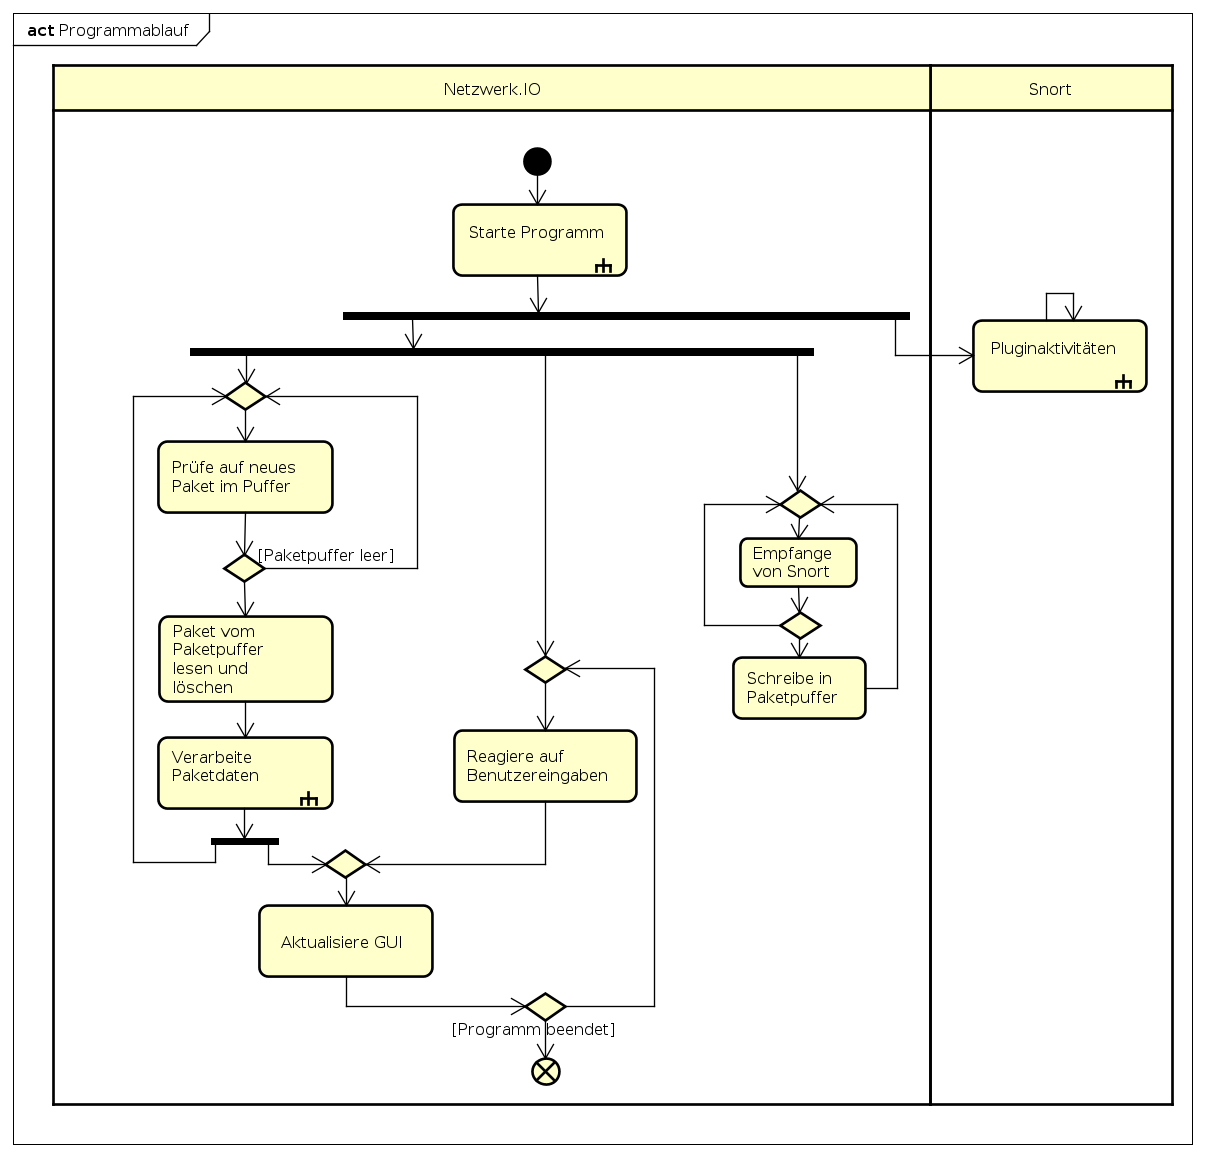
\includegraphics[width=\textwidth]{../diagrams/AD_Programmablauf}


\pagebreak
\subsection{Beschreibung: Starte Programm}
	
	\begin{easylist}[enumerate]
	\ListProperties(Style2*=,Numbers=a,Numbers1=R,FinalMark1={.},FinalMark2={.},FinalMark3={.},Numbers4=l)
	
	
	& Initialisiere relevante Daten
	
	& Wenn Snort noch nicht läuft, frage den Benutzer ob Snort gestartet werden soll
		&& Wenn der Benutzer zustimmt wird Snort mit Plugin gestartet
		&& Wenn der Benutzer ablehnt wird Netzwerk.IO beendet
	
	& Wenn Snort schon läuft, dann Benutzer fragen ob Plugin gestartet werden soll
	    && Wenn der Benutzer zustimmt wird Snort mit dem Plugin neu geladen
	    && Wenn der Benutzer nicht zustimmt wird Netzwerk.IO beendet
	
	\end{easylist}
	
	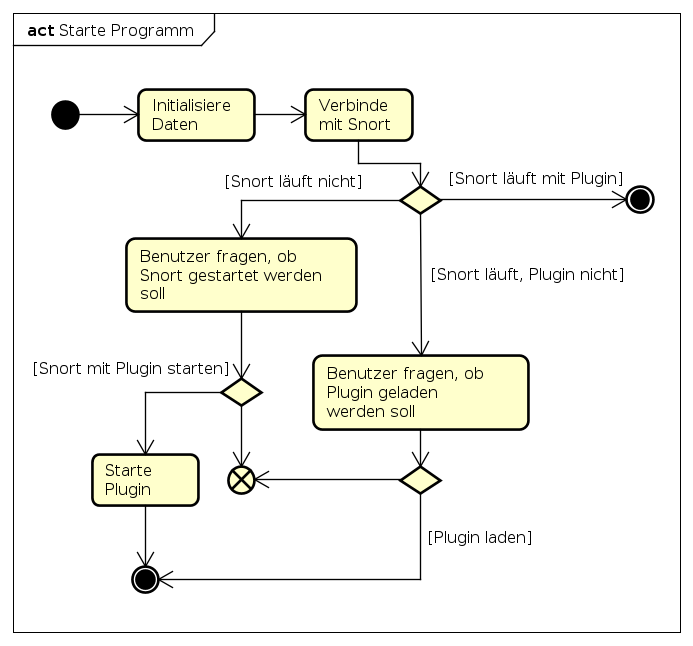
\includegraphics[width=\textwidth]{../diagrams/AD_Starte_Programm}

\pagebreak
\subsection{Beschreibung: Pluginaktivitäten}

	\begin{easylist}[enumerate]
	\ListProperties(Style2*=,Numbers=a,FinalMark1={.},FinalMark2={.},FinalMark3={.},Numbers4=l)
	
	
	& Das Snort Plugin empfängt ein neues Paket
	& Das Paket wird dekodiert
	& Das dekodierte Paket wird auf Fehler geprüft
	    && Wenn ein Fehler gefunden wurde wird das Paket als fehlerhaft markiert
	& Das Paket wird an Netzwerk.IO weitergesendet
	& Das Paket wird für weitere Analysen auch an Snort weitergegeben
	
	\end{easylist}
	
	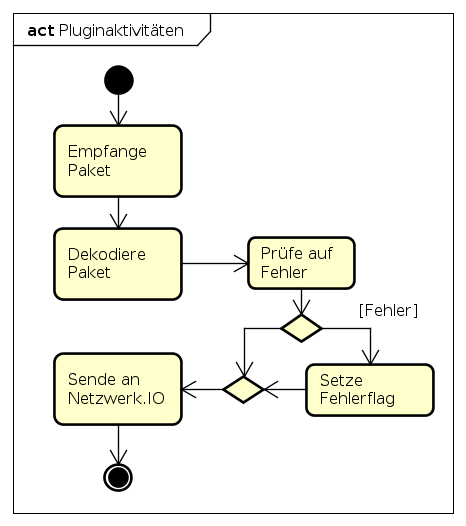
\includegraphics[width=0.5\textwidth]{../diagrams/AD_Pluginaktivitaeten}

\pagebreak
\subsection{Beschreibung: Verarbeite Paketdaten}

	\begin{easylist}[enumerate]
	\ListProperties(Style2*=,Numbers=a,Numbers1=R,FinalMark1={.},FinalMark2={.},FinalMark3={.},Numbers4=l)
	
	
	& Das Snort Plugin empfängt ein neues Paket
	& Das Paket wird dekodiert
	& Das dekodierte Paket wird auf Fehler geprüft
	    && Wenn ein Fehler gefunden wurde wird das Paket als fehlerhaft markiert
	& Das Paket wird an Netzwerk.IO weitergesendet
	& Das Paket wird für weitere Analysen auch an Snort weitergegeben
	
	\end{easylist}
	
	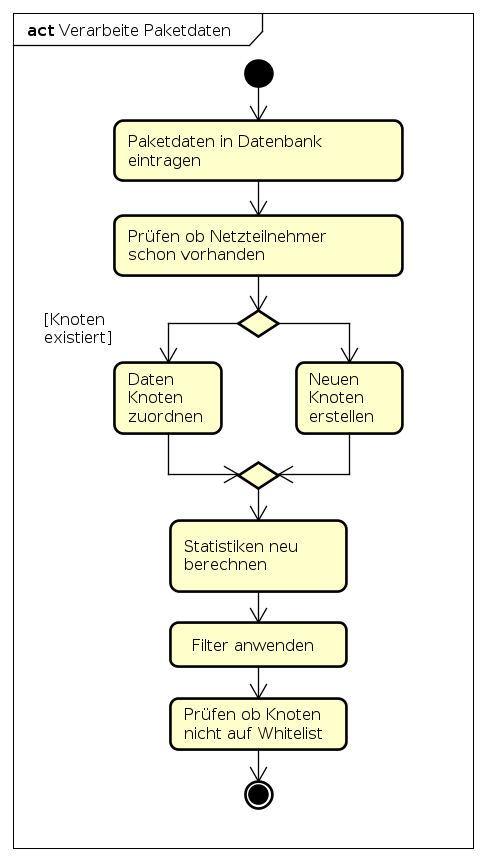
\includegraphics[width=0.5\textwidth]{../diagrams/AD_Verarbeite_Paketdaten}
